%% Projective Incidence Calculus for Transformer Decision Logic
%% ACM sigconf submission. Build: pdflatex pic && bibtex pic && pdflatex pic && pdflatex pic
%%
%% Uses [nonacm] so the draft compiles without the venue's rights block; at
%% camera-ready remove `nonacm`, add the venue's \acmConference / \setcopyright /
%% \acmDOI lines, and (for double-blind review) add `anonymous,review`.
\documentclass[sigconf,nonacm]{acmart}

\settopmatter{printacmref=false}
\setcopyright{none}
\renewcommand\footnotetextcopyrightpermission[1]{}

\usepackage{booktabs}
\usepackage{amsmath}
\usepackage{tikz}
\usetikzlibrary{positioning,arrows.meta,fit,backgrounds}
% NB: do not load amssymb here -- acmart's newtxmath already defines \Bbbk etc.
% (\mathbb and the symbols used in this paper come from acmart's math font).

\newtheorem{theorem}{Theorem}
\newtheorem{lemma}{Lemma}
\newtheorem{corollary}{Corollary}
\theoremstyle{definition}
\newtheorem{definition}{Definition}

% allow a little extra slack to avoid small overfull boxes in math-heavy lines
\setlength{\emergencystretch}{1em}

% notation (\H is predefined as the Hungarian-umlaut accent -> renew, not new)
\newcommand{\R}{\mathbb{R}}
\renewcommand{\H}{\mathcal{H}}
\newcommand{\D}{\mathcal{D}}
\newcommand{\inner}[2]{\langle #1, #2\rangle}
\newcommand{\Uv}{U_v}
\renewcommand{\dj}{d_j}  % \dj is predefined (the d-stroke char) -> renew
\newcommand{\nb}{n_b}
% status tags for results
\newcommand{\proved}{\textsc{[proved]}}
\newcommand{\measured}{\textsc{[measured]}}
\newcommand{\open}{\textsc{[open]}}

\begin{document}

\title{Projective Incidence Calculus for Transformer Decision Logic}

\author{J. Allan Scott}
\affiliation{%
  \institution{Independent Researcher}
  \city{Concord}
  \state{New Hampshire}
  \country{USA}}
\email{allan@jallan.scot}

\renewcommand{\shortauthors}{J. Allan Scott}

\begin{abstract}
We introduce \emph{Projective Incidence Calculus} (PIC), a geometric formalism that
models transformer decision logic as signed evidence accumulation in a Hilbert
space, and use it as a principled \emph{diagnostic lens} on real models. PIC turns
the additive read-out into measurable structure. Applying it to
direct-logit-attribution dumps from the \texttt{fieldrun} probing infrastructure on
\emph{two model families}---Qwen2.5 (0.5B--3B) and Pythia (70M--1B)---we find that
routing is strongly \emph{rank-concentrated} in both: the decode rides a stable,
late-layer, MLP-dominated circuit using far fewer effective blocks than are
available. \emph{Coherence packing, by contrast, is family-dependent.} Qwen routing
features sit 2--3$\times$ above the information-theoretic (Welch) floor, whereas
Pythia packs near-optimally (1.06--1.5$\times$); at matched dimension ($\nb{=}49$),
Pythia-410M (1.38$\times$) is markedly tighter than Qwen2.5-0.5B (2.01$\times$),
showing that near-Welch-optimal packing is achievable in general pretraining and is
\emph{not} limited to task-specialized regimes. These are structural properties of
routing invisible to accuracy or loss curves.
%
The formalism rests on a machine-checked backbone: PIC modernizes classical
incidence calculus (set-based incidences become inner products, structural overlap a
Gram kernel) and connects the hard ($T{=}0$) decision surface to tropical geometry
via Laguerre power diagrams. On this base we define \emph{Tropical Realization
Complexity} (TRC), the cost of routing inputs into the correct cells, and prove its
core results: exact softmax/decode recovery, a decode-separation lemma with a
$\gamma$-code packing bound, and a generator-rank bound.
%
On a controlled synthetic substrate, four theory-guided interventions all fail to
outperform plain gradient descent. These results are clarifying: they show that the
framework's value is diagnostic rather than algorithmic, because (i) the capacity
bound is slack by $\sim$50--59 orders of magnitude, (ii) realization cost is
dominated by the number of trainable generators, not the number of routing
decisions---a \emph{superposition} quantity---and (iii) gradient descent already
packs routing features near the Welch floor when given a well-defined task. We
release the \texttt{fieldrun}
infrastructure, the \texttt{i-orca} machine-checked certificate corpus, and the
\texttt{pil} learning code.
\end{abstract}

\begin{CCSXML}
<ccs2012>
<concept><concept_id>10010147.10010257</concept_id><concept_desc>Computing methodologies~Machine learning</concept_desc><concept_significance>500</concept_significance></concept>
<concept><concept_id>10003752.10003790</concept_id><concept_desc>Theory of computation~Logic</concept_desc><concept_significance>300</concept_significance></concept>
</ccs2012>
\end{CCSXML}
\ccsdesc[500]{Computing methodologies~Machine learning}
\ccsdesc[300]{Theory of computation~Logic}

\keywords{transformers, tropical geometry, incidence calculus, mechanistic
interpretability, routing, superposition, formal verification}

\maketitle

\section{Introduction}

A decoder transformer~\cite{vaswani2017attention} predicts the next token by
iteratively writing additive contributions into a residual stream and reading the
result through an unembedding matrix. This additive structure is well understood at
the level of implementation: every layer, attention head, and MLP block adds a
vector, and the logits are a linear read-out of the sum. What has been missing is a
unified \emph{geometric and logical} account of how those contributions combine
into a \emph{confident decision}---and a precise statement of what limits the
confident decisions a given read-out geometry can support.

We propose such an account. \emph{Projective Incidence Calculus} (PIC) treats each
residual contribution as casting a vector of signed \emph{incidences} (inner
products) onto a frame of proposition directions, the unembedding rows. The decode
is the tropical ($\max$-plus) collapse of the accumulated incidences, and its
geometry is a Laguerre power diagram. PIC recovers the softmax exactly at
temperature $T{=}1$ and the greedy decode at $T{=}0$; the two live in one program
under two semirings. On this base we define \emph{Tropical Realization Complexity}
(TRC), a measure of the cost of routing a data distribution into the correct cells.

The payoff of this geometry is \emph{measurement}. PIC names quantities---rank
concentration, the read-out circuit, coherence relative to the Welch floor,
difficulty-driven fallback---that a practitioner can read off a frozen model and
that behave lawfully across scale, language, and difficulty (\S\ref{sec:real}).
\emph{While PIC and TRC do not yield superior training algorithms in the regimes we
tested, they provide a principled diagnostic lens that reveals structural properties
of real-model routing invisible to standard accuracy or loss curves.} That is the
paper's main claim, and it is what the rest of the contributions support.

To establish where the framework measures rather than optimizes, we use a learning
system, \emph{Projective Incidence Learning} (PIL), which owns and updates the
proposition frame and a bank of generated rules. On controlled substrates with a
\emph{known} ground-truth factorization, PIL lets us ask which parts of the theory
are levers for training and which are only good for measurement. The answer is
sharp---and the clarifying negative results (\S\ref{sec:nulls}) are precisely what
make the positive real-model findings interpretable.

Throughout we separate three epistemic statuses and tag every claim accordingly, so
that the formal and empirical content never blur: \proved{} (machine-checked
end-to-end, with no admitted steps, in the companion \texttt{i-orca}
corpus~\cite{iorca}), \measured{}
(empirical, this work or \texttt{fieldrun}), and \open{} (conjecture). The paper's
arc is measure-first: define the diagnostics, validate them on two real model
families, and use a controlled synthetic substrate to show \emph{why} they are
diagnostics rather than training levers. Concretely, our contributions are:

\begin{itemize}
\item \textbf{A formal geometric model of transformer decision logic}
(\S\ref{sec:pic}) grounded in incidence calculus and tropical geometry, with three
machine-checked structural results: exact softmax/decode recovery, a decode
\emph{separation} lemma yielding a $\gamma$-code packing bound on confidently
decodable tokens, and a generator-rank bound.
\item \textbf{Tropical Realization Complexity} (\S\ref{sec:trc}) and the empirical
finding (\S\ref{sec:routing}) that it is a \emph{superposition-capacity} quantity:
realization cost scales with the number of trainable generators, not the number of
routing decisions, and the binding constraint in practice is per-example routing,
not cell capacity (which is slack by $\sim$50--59 orders).
\item \textbf{A set of clarifying controls} (\S\ref{sec:synthetic}): four
theory-guided interventions---frame regularization, min-margin rule targeting,
propose-score-select, and a generator coherence penalty---each fail to beat plain
gradient descent, because SGD already packs routing features near the Welch floor.
This delimits where the theory is, and is not, an algorithm.
\item \textbf{A two-family real-model validation} (\S\ref{sec:real}) over Qwen2.5
(0.5B--3B)~\cite{qwen2025} and Pythia (70M--1B)~\cite{biderman2023pythia}, plus a
difficulty dial and (in the appendix) five languages: rank concentration on a stable
late-MLP circuit transfers to both families, while coherence packing is
\emph{family-dependent}---Qwen sits 2--3$\times$ above the Welch floor and Pythia
packs near it, refuting the prior reading that near-optimal packing is
synthetic-specific.
\item \textbf{Open-source tooling}: the \texttt{fieldrun}
\texttt{-{}-pil-dump}~\cite{fieldrun} direct-logit-attribution seam, the
\texttt{i-orca} certificate corpus~\cite{iorca}, and the \texttt{pil} learning
code~\cite{pil}, with every figure regenerable from checked-in result files.
\end{itemize}

\section{Background}

\subsection{Transformers and direct logit attribution}
A transformer maintains a residual stream that is the running sum of additive
contributions: an embedding, and, per layer, one attention output and one MLP
output. Writing $U$ for the unembedding, the final logit of token $v$ is
$L_v=\inner{r}{\Uv}+b_v$ where $r$ is the final residual. Because $r=\sum_j \dj$ is
a sum, $L_v=\sum_j\inner{\dj}{\Uv}+b_v$ decomposes \emph{exactly} into per-block
contributions. This is \emph{direct logit attribution} (DLA): the contribution
$\inner{\dj}{\Uv}$ of block $j$ to token $v$~\cite{elhage2021framework,
nostalgebraist2020logitlens}. We take the additive blocks
($\nb=2L{+}1$ for an $L$-layer model) as the atomic ``circuits'' and their
per-candidate contributions as the incidences.

\subsection{Incidence calculus}
Classical incidence calculus~\cite{bundy1985incidence,liu1996incidence} attaches to
each proposition the \emph{set of possible worlds (incidences)} in which it holds,
and computes with these sets rather than with scalar probabilities alone. This
preserves the dependencies that a purely numeric calculus discards and handles
non-truth-functional combination faithfully. PIC keeps the spirit---propositions
carry structured \emph{evidence} that combines, not just a number---but replaces the
Boolean lattice of world-sets with the inner-product geometry of a Hilbert space,
so that ``incidence'' becomes a signed real (a DLA term) and ``structural overlap''
becomes a Gram entry.

\subsection{Tropical geometry and neural networks}
Zhang, Naitzat, and Lim~\cite{zhang2018tropical} showed that feedforward ReLU
networks are tropical rational maps: decision boundaries are tropical hypersurfaces
and linear regions correspond to vertices of an associated Newton polytope. This has
been extended to real tropical geometry~\cite{brandenburg2024real}, decision-boundary
analysis~\cite{alfarra2023decision}, and linear-region
counting~\cite{montufar2014regions,serra2018regions}. We apply these ideas not to a
feedforward classifier but to the \emph{routing/decode} behavior of a transformer
read-out, where the relevant tropical object is the upper envelope of the affine
logit functions---a Laguerre power diagram~\cite{maclagan2015tropical}.

\section{Projective Incidence Calculus}
\label{sec:pic}

PIC models the transformer read-out in a Hilbert space $\H=\R^d$. Sources (circuits
/ partial evidence) are vectors $\dj\in\H$; the proposition frame
$U=\{\Uv\}_{v\in V}\subset\H$ is the set of unembedding rows.
Table~\ref{tab:proved} lists the formal backbone established in this section and the
next; it is the load-bearing distinction of the paper, so we state it once, up
front---these results are \proved, everything in
\S\ref{sec:synthetic}--\ref{sec:real} is \measured.

\begin{table}[t]
\caption{The machine-checked backbone of PIC and TRC (all \proved, with no admitted
steps, in the \texttt{i-orca} corpus~\cite{iorca}). Empirical claims are tagged
\measured{} in situ; conjectures \open.}
\label{tab:proved}
\small
\begin{tabular}{@{}lp{0.60\columnwidth}@{}}
\toprule
result & one-line statement \\
\midrule
Softmax recovery (Thm.~\ref{thm:softmax}) & product-of-experts over incidences $=$ softmax at $T{=}1$, greedy decode at $T{=}0$ \\
Decode separation (Thm.~\ref{thm:sep}) & two $\gamma$-decodable tokens have frames $\ge\gamma$ apart; biases cancel \\
$\gamma$-code packing (Cor.~\ref{cor:packing}) & at most $(1+2\rho/\gamma)^d$ confidently decodable tokens fit in $\R^d$ \\
Generator rank (Thm.~\ref{thm:rank}) & $M$ generators move the logits within a $\le\min(M,d)$-dim.\ subspace \\
Routing Welch (Thm.~\ref{thm:welch}) & $n>m$ routing features in $\R^m$ force coherence $\ge$ the Welch floor \\
\bottomrule
\end{tabular}
\end{table}

\begin{definition}[Incidence]
The incidence of source $\dj$ on proposition $\Uv$ is the inner product
$c_j^v=\inner{\dj}{\Uv}$ (the DLA term).
\end{definition}

\begin{definition}[Aggregate logits]
With $r=\sum_j \dj$, the logit of $v$ is
$L_v=\inner{r}{\Uv}+b_v=\sum_j c_j^v+b_v.$
\end{definition}

\begin{definition}[Gram kernel]
Structural overlap between propositions is the Gram matrix
$G_{vw}=\inner{\Uv}{U_w}$. High $|G_{vw}|$ is the near-synonym / common-mode regime
in which differential evidence collapses; a diagonal $G$ is the classical
(Boolean-incidence) limit.
\end{definition}

\paragraph{Two algebras.}
The model factors into an \emph{inner, linear} algebra---accumulation
$r=\sum_j \dj$ and attribution $c_j^v=\inner{\dj}{\Uv}$ are entirely
linear/bilinear---and an \emph{outer, tropical} algebra: the decode
$\hat v=\arg\max_v L_v$ is a $\max$-plus collapse. The first result makes the bridge
exact.

\begin{theorem}[Softmax/decode recovery; \proved, \texttt{i-orca}: \texttt{RecoveredProbability}]
\label{thm:softmax}
The product-of-experts model whose per-source likelihoods are the exponentiated
incidences returns exactly the transformer softmax at temperature $T{=}1$, and the
greedy $\arg\max$ decode at $T{=}0$. The same program is sound under both the
log-semiring and the tropical ($\max$-plus) semiring (a Maslov sandwich).
\end{theorem}

\paragraph{The tropical decision surface.}
At $T{=}0$ the hard decision $\arg\max_v L_v$ is governed by the tropical polynomial
$M(r)=\max_v\bigl(\inner{r}{\Uv}+b_v\bigr)$. Its regions are the cells of a
\emph{Laguerre power diagram} with additive weights $\|\Uv\|^2-2b_v$: the decision
region of $v$ is $C_v=\{r:L_v\ge L_w~\forall w\}$, and the normalized decode margin
is the (signed) distance from $r$ to the nearest cell facet. This is the
transformer-routing instance of the ReLU-as-tropical-rational
picture~\cite{zhang2018tropical,maclagan2015tropical}.

\paragraph{How many confident decodes fit?}
The central structural question is: given a frame in $\R^d$, how many tokens can be
decoded with a guaranteed margin? Call $v$ \emph{$\gamma$-decodable} if some unit
residual ($\|r\|\le1$) decodes to $v$ with margin $\ge\gamma$. The answer is a clean
separation lemma whose proof cancels the biases.

\begin{theorem}[Decode separation; \proved, \texttt{i-orca}: \texttt{DecodeCapacity}]
\label{thm:sep}
If $v\ne w$ are both $\gamma$-decodable, then $\|\Uv-U_w\|\ge\gamma$,
\emph{independent of the biases} $b$.
\end{theorem}

\begin{proof}[Proof sketch]
Let $r_v,r_w$ be the unit witnesses. Margin $\ge\gamma$ at $r_v$ gives
$\inner{r_v}{\Uv-U_w}+(b_v-b_w)\ge\gamma$, and symmetrically
$\inner{r_w}{U_w-\Uv}+(b_w-b_v)\ge\gamma$. Adding cancels the biases:
$\inner{r_v-r_w}{\Uv-U_w}\ge2\gamma$. Cauchy--Schwarz with
$\|r_v-r_w\|\le2$ yields $\|\Uv-U_w\|\ge\gamma$.
\end{proof}

\begin{corollary}[$\gamma$-code packing bound]
\label{cor:packing}
The $\gamma$-decodable set is a $\gamma$-separated code in $\R^d$, so by sphere
packing
$N_\gamma\le\bigl(1+\tfrac{2\rho}{\gamma}\bigr)^{d}$, with $\rho=\max_v\|\Uv\|$.
\end{corollary}

This is the decision-side sibling of the Welch bound: Welch~\cite{welch1974lower}
bounds the \emph{coherence} of $V$ vectors in $\R^d$; Corollary~\ref{cor:packing}
bounds the \emph{count} of $\gamma$-separated decodes. Both are packing statements.
A companion \texttt{HeadTail} certificate shows that a compact ``head'' of
propositions reproduces the full decode \emph{iff} it tropically dominates the
remaining ``tail,'' and that the certifiable head is itself capacity-bounded by
Corollary~\ref{cor:packing}---the tail is the explicit irreducible residue (the
``forge tax'' of open-class tokens).

\paragraph{Adjustments are low-rank.}
Finally, when the read-out is augmented by $M$ trainable generators (rules), the set
of achievable logit \emph{adjustments} is constrained.

\begin{theorem}[Generator rank; \proved, \texttt{i-orca}: \texttt{RoutingRank}]
\label{thm:rank}
The logit adjustments realizable by $M$ generators lie in a subspace of dimension at
most $\min(M,d)$. When the number of routing features to be distinguished exceeds
this rank, superposition is forced.
\end{theorem}

\section{Tropical Realization Complexity}
\label{sec:trc}

\begin{definition}[Tropical Realization Complexity]
\label{def:trc}
The TRC of a data distribution $\D$ at margin $\gamma$ and interference tolerance
$\varepsilon$ is the minimal number $M$ of trainable generators that route $\D$ into
the correct power-diagram cells with margin $\ge\gamma$ and routing-feature
interference $\le\varepsilon$.
\end{definition}

\begin{figure}[t]
\centering
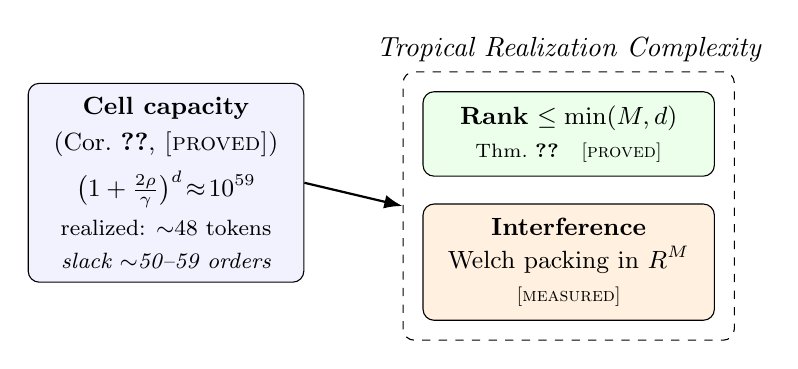
\begin{tikzpicture}[font=\small,
  box/.style={draw, rounded corners, align=center, inner sep=5pt},
  capbox/.style={box, fill=blue!5, minimum width=3.5cm, minimum height=2.4cm},
  sub/.style={box, minimum width=3.7cm, minimum height=1.0cm}]
\node[capbox] (c) {\textbf{Cell capacity}\\[2pt](Cor.~\ref{cor:packing}, \proved)\\[4pt]
  $\big(1+\tfrac{2\rho}{\gamma}\big)^{d}\!\approx\!10^{59}$\\[3pt]
  \footnotesize realized: $\sim$48 tokens\\[1pt]
  \footnotesize\itshape slack $\sim$50--59 orders};
\node[sub, fill=green!8] (r) [right=1.5cm of c, yshift=0.62cm]
  {\textbf{Rank} $\le\min(M,d)$\\[1pt]\scriptsize Thm.~\ref{thm:rank}\quad\proved};
\node[sub, fill=orange!12] (i) [below=0.34cm of r]
  {\textbf{Interference}\\[1pt]Welch packing in $\R^{M}$\\[1pt]\scriptsize\measured};
\begin{scope}[on background layer]
\node[draw, dashed, rounded corners, fit=(r)(i), inner sep=7pt,
  label={[font=\itshape]above:Tropical Realization Complexity}] (trc) {};
\end{scope}
\draw[-{Latex}, thick] (c.east) -- (trc.west);
\end{tikzpicture}
\caption{Cell capacity vs.\ Tropical Realization Complexity. The $\gamma$-code
packing bound permits $\sim$$10^{59}$ confident decodes but only $\sim$48 are
realized---capacity is not the binding limit. TRC is: a \proved\ rank budget
($\le\min(M,d)$) plus a \measured\ interference term that is a Welch packing of
routing features into $\R^{M}$ (rule-activation space), set in practice by
per-example routing.}
\label{fig:trc}
\end{figure}

TRC decomposes into two components with very different epistemic status.

\paragraph{Rank component (\proved).}
By Theorem~\ref{thm:rank}, $M$ generators move the logits within a
$\le\min(M,d)$-dimensional subspace. If a task requires distinguishing more
routing features than this rank, they must share dimensions---superposition is
unavoidable. This is the dimension budget of TRC.

\paragraph{Interference component (\measured/\open).}
Within the available rank, packing $n$ routing features incurs mutual coherence.
The structural floor is provable: for $n$ unit features in $m$ dimensions with
$n>m$, mean-squared coherence is $\ge(n-m)/(m(n-1))$.

\begin{theorem}[Routing Welch floor; \proved, \texttt{i-orca}: \texttt{RoutingWelch}]
\label{thm:welch}
$n>m$ unit routing features in $\R^m$ have mean-squared coherence at least the Welch
bound $(n-m)/(m(n-1))$; equality requires an equiangular tight frame.
\end{theorem}

We deliberately do \emph{not} promote the floor to a margin-degradation
\emph{law}. Our measurements (\S\ref{sec:routing}) show the coherence$\to$margin
link is empirically mild; asserting a clean $\gamma\le\gamma_0(1-c\mu)$ theorem would
contradict the data.

\smallskip
\noindent\fbox{\parbox{0.94\columnwidth}{\small\textbf{Empirical correction
(\S\ref{sec:routing}).} The packing dimension for the interference term is $M$---the
\emph{rule-activation} space---\textbf{not} $\min(M,d)$. This is the single most
important refinement to Definition~\ref{def:trc}: TRC is a Welch packing of $n$
routing features into $M$ dimensions, and interference appears precisely when
$n>M$.}}
\smallskip

\section{Experiments: synthetic substrate}
\label{sec:synthetic}

We construct synthetic problems with a \emph{known} ground-truth factorization so
that ``which lever matters'' has a checkable answer. The model owns a proposition
frame $U$ and (optionally) a bank of ReLU rules $h_k(z)=\mathrm{relu}(\inner{w_k}{z}+b_k)$
emitted as extra sources. Every loss term is labelled \emph{decode-side} (the NLL
and a worst-competitor hinge margin---exactly what \texttt{fieldrun} measures on a
frozen model) or \emph{frame-side} (the frame potential, mean-squared off-diagonal
cosine, driven toward the Welch floor). Unless noted, evaluation is on a held-out
25\% split and results are averaged over 2--3 seeds.

The section answers one question---\emph{which lever moves the decode?}---in three
moves. \S\ref{sec:frame}--\ref{sec:generation} contrast the two candidate levers
(frame geometry vs.\ generation), finding only generation works.
\S\ref{sec:scored}--\ref{sec:routing} then show \emph{why} the theory's refinements
of generation do not help: capacity does not bind, and realization cost is an
$M$-dominated superposition quantity. \S\ref{sec:nulls} collects the resulting four
nulls, the section's highest-signal takeaway.

\subsection{Frame optimization is decoupled from the decode}
\label{sec:frame}
We first test the most natural ``geometric'' lever: regularize the frame to be more
incoherent. We use an 8$\times$ over-complete regime ($d{=}24$, $V{=}192$, 24 planted
synonym clusters, within-cluster $|\cos|{=}0.82$, Welch floor $0.037$). It behaves as
designed: synonymy compresses margins so hard that retrievability is $0.40$ while
top-1 accuracy is $0.99$, and the strongest competitor is a synonym 88\% of the time. Sweeping the frame-potential weight \emph{does} move the frame
geometry (frame potential $1.35\to1.09\times$ Welch) but leaves \emph{every} decode
metric flat (Table~\ref{tab:frame}). Across the entire synonymy$\times$noise plane,
$|\Delta\text{retr}|\le0.01$ while the baseline retrievability swings $0.02\to0.80$
under the real levers (synonymy spread and source SNR). The frame regularizer is
\emph{redundant} where the margin term already shapes the frame and \emph{impotent}
where the bottleneck is source distinguishability: when synonyms have near-identical
sources, the margin is source-SNR-bound, and no read-out objective can manufacture
absent signal.

\begin{table}[t]
\caption{Frame regularization is decoupled from the decode (hard over-complete
regime, $d{=}24$, $V{=}192$, 3 seeds). The frame potential moves; the decode does
not.}
\label{tab:frame}
\small
\begin{tabular}{lccccc}
\toprule
\texttt{frame\_reg} & retr & top1 & margin & nll & fp/Welch \\
\midrule
0.00 & 0.395 & 0.99 & 1.240 & 1.949 & 1.346 \\
0.10 & 0.400 & 0.99 & 1.241 & 1.949 & 1.244 \\
0.50 & 0.395 & 0.99 & 1.242 & 1.948 & 1.094 \\
\bottomrule
\end{tabular}
\end{table}

\subsection{Generation is the lever}
\label{sec:generation}
\S\ref{sec:frame} says the bottleneck is generative, not the frame. We test this
directly with a compositional regime: synonyms share a one-hot \emph{topic} atom (so
they collide on $r$), and a fraction of clusters are \emph{hard}---the synonym is the
\emph{XOR} of two code atoms, provably not linearly separable---while the rest are
\emph{easy} (parity read directly). A frame-only model is a linear read-out and is
pinned at chance on the hard clusters (within-synonym accuracy $0.454$, margin
$\approx0$). Adding generated ReLU rules lifts hard-cluster accuracy to $0.93$
(Fig.~\ref{fig:lever}). A \texttt{signal=False} control (parity is noise) collapses
all arms to chance, confirming the honest boundary: generation recovers signal only
when it exists.

\begin{figure}[t]
\centering
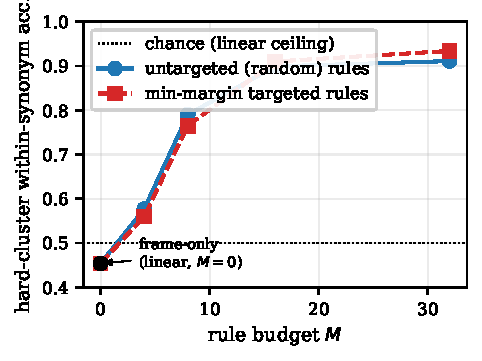
\includegraphics[width=0.92\columnwidth]{figures/generation_lever.pdf}
\caption{Generation is the lever; targeting is not. A frame-only linear read-out is
pinned at chance on the XOR-coded hard clusters ($M{=}0$); generated rules lift
hard-cluster within-synonym accuracy to $0.93$. Min-margin targeting (dashed) is
statistically indistinguishable from random rules (solid)---SGD already allocates
rules to the at-risk facets.}
\label{fig:lever}
\end{figure}

But the second half is a null. \emph{Min-margin-targeted} rule placement---seeding
rules at the at-risk facets discovered from a frame-only warmup---barely beats
\emph{random} rules ($0.934$ vs.\ $0.911$ at budget $32$; behind at low budget). The
mechanism is clear: gradient descent already drives hidden units to the hard
clusters, so explicit targeting buys initialization, not allocation.

\subsection{Selection is not the lever; capacity does not bind}
\label{sec:scored}
To separate ``proposal quality'' from ``trained vs.\ frozen feature,'' we cross a
selection method (random, variance, $\eta^2$-on-ambiguous-examples) with
frozen vs.\ trainable input weights (Table~\ref{tab:scored}). The split is
\emph{entirely} along frozen-vs-trainable: making the scored arm trainable jumps it
from $0.53$ to $0.74$ at $M{=}8$, matching SGD, while every frozen arm stalls. Once
rules are trained, theory-guided selection is indistinguishable from random
initialization; once frozen, no selection rescues them.

\begin{table}[t]
\caption{The decisive 2$\times$2: training, not selection, is the lever
(hard-cluster within-synonym accuracy, held-out, 3 seeds, chance $0.5$). The
\texttt{code} column is the realized $\gamma$-separated code (clusters with both
synonyms confidently decoded; max 24).}
\label{tab:scored}
\small
\begin{tabular}{lccccc}
\toprule
$M$ & sgd & ambig-frozen & ambig-train & rand-frozen & rand-train \\
\midrule
8  & 0.722 & 0.532 & \textbf{0.741} & 0.540 & \textbf{0.750} \\
16 & 0.859 & 0.579 & 0.852 & 0.632 & 0.854 \\
32 & 0.905 & 0.684 & 0.891 & 0.668 & 0.873 \\
\midrule
code & 24 & 24 & 24 & 24 & 24 \\
\bottomrule
\end{tabular}
\end{table}

Critically, the structural metric \emph{saturates}: even frozen rules at $0.58$
accuracy realize the full $\gamma$-separated code ($24/24$ clusters). Quantifying
this against Corollary~\ref{cor:packing} ($d{=}32$, $V{=}48$): the realized code is
$48/48$ tokens, while the packing bound is $\sim10^{59}$ at $\gamma{=}1$ (and
$\sim10^{51}$ at $\gamma{=}1.8$). \emph{Capacity is thus slack by $\sim$50--59 orders
of magnitude.} The minimum frame separation inside the code ($0.90$) further exceeds
the effective $\gamma$ by $17$--$31\times$. So creating new $\gamma$-separated
high-margin tokens is not the bottleneck; that capacity is realized with enormous
slack. The binding constraint is per-example routing: getting the \emph{right} decode
for \emph{each} input, which is a training problem, not a capacity or selection one.

\subsection{Realization cost is $M$-dominated---a superposition quantity}
\label{sec:routing}
We next operationalize TRC. Holding cell capacity fixed (slack $\sim10^{59}$), we
vary the number of independent non-linear routing decisions $n_\text{hard}$ and the
rule budget $M$ (Fig.~\ref{fig:mdom}). The natural hypothesis---accuracy is governed
by rules-per-decision $M/n_\text{hard}$---is \emph{refuted}: accuracy depends on the
absolute budget $M$ and essentially not on $n_\text{hard}$. At $M{=}8$ all of
$n_\text{hard}\in\{4,\dots,24\}$ reach $\sim0.76$; at $M{=}32$ all reach $\sim0.91$.
The minimal $M$ to reach $0.85$ is $\sim$16--32 regardless of $n_\text{hard}$, so
$M^\star/n_\text{hard}$ \emph{falls} from $4.0$ to $0.67$: 24 disjoint XOR routings
need no more rules than 4.

\begin{figure}[t]
\centering
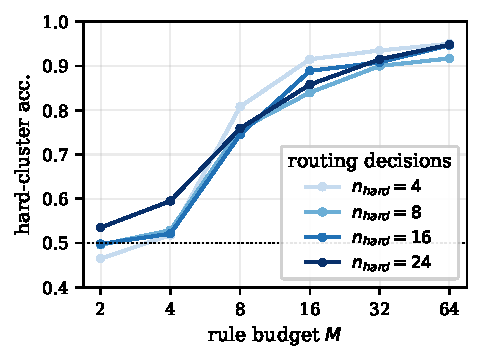
\includegraphics[width=0.92\columnwidth]{figures/m_dominance.pdf}
\caption{Realization cost is dominated by the rule budget $M$, not the number of
routing decisions $n_\text{hard}$: the curves collapse against $M$, not against
$M/n_\text{hard}$. The $M$ rules represent the $n_\text{hard}$ routing features in
\emph{superposition}.}
\label{fig:mdom}
\end{figure}

The interpretation is superposition: the $M$ rules represent the $n_\text{hard}$
routing features amortized across decisions, with accuracy set by how many features
$M$ rules can disentangle, not by the decision count. \textbf{TRC is therefore a
superposition-capacity quantity}, not a per-decision count---the same superposition
the broader program studies, now on the routing side.

This reframes the interference term. Probing the margin and the realized coherence
$\mu$ of the per-cluster routing directions (Table~\ref{tab:interf}) gives three
readings. First, there is no clean Welch-degradation cliff: $M{=}16$ is flat, and
$M{=}8$ declines only $\sim$13\%. Second, the relevant dimension in
Theorem~\ref{thm:welch} is $M$, not $\min(M,d)$---the routing features live in
\emph{rule-activation space} $\R^M$, so interference appears precisely when
$n_\text{hard}>M$, where $\mu$ sits at the Welch floor. Third, training packs
near-optimally: realized $\mu$ tracks the floor without wildly exceeding it, so
exceeding $M$ costs only mild margin, not failure. A direct generator-side coherence
regularizer confirms the picture---it lowers $\mu$ on target but leaves margin and
accuracy flat ($|\Delta\text{margin}|\le0.04$), even at 2--3$\times$ over-packing.

\begin{table}[t]
\caption{Interference is mild and lives in $\R^M$ (held-out, 3 seeds, $d{=}32$).
Coherence $\mu$ reaches the Welch floor only once $n_\text{hard}>M$; the margin
degrades only weakly there.}
\label{tab:interf}
\small
\begin{tabular}{llccc}
\toprule
$M$ & margin ($n{=}1\!\to\!24$) & $\mu$ & Welch ($n{=}24$) & verdict \\
\midrule
8  & $2.10\to1.83$ & $\sim$0.28 & 0.295 & mild, only $n{>}M$ \\
16 & $2.93\to3.11$ & $\sim$0.19 & 0.147 & no degradation \\
\bottomrule
\end{tabular}
\end{table}

\subsection{Four nulls, one lesson}
\label{sec:nulls}
Four theory-guided knobs have now been tested against plain end-to-end SGD
(Table~\ref{tab:nulls}); none beats it. The consistent lever is simply
$M\ge$ the effective rank of the routing features, with SGD packing them near the
Welch floor on its own. This is also why a coherence$\to$margin degradation theorem
is not worth formalizing: coherence is real and Welch-floored (Theorem~\ref{thm:welch}),
but it is empirically decoupled from the margin. The honest theory boundary is that
the \emph{structural packing bounds are provable} (and proved), while the
\emph{margin consequence} is mild and not a clean law.

\paragraph{Why this calibrates the real-model results.}
These nulls are not a dead end; they are the measuring stick for
\S\ref{sec:real}. Because SGD packs near the Welch floor whenever it is \emph{trained
on a task}, tight routing has a known signature---rank used up, coherence
$\sim$1$\times$ the floor. Any slack a \emph{pretrained} model shows against that
signature (rank left unused, coherence above the floor) is therefore not an
optimization failure but a structural fact about a model that was never specialized
to a single routing decomposition. The synthetic regime fixes the reference point so
that the real-model departures from it are interpretable rather than arbitrary.
\emph{In one line: wherever SGD can reach, the theory's role is to bound and measure
the packing, not to improve it.}

\begin{table}[t]
\caption{The symmetry closes: four theory-guided interventions, all null vs.\ SGD.}
\label{tab:nulls}
\small
\begin{tabular}{lll}
\toprule
knob & side & result \\
\midrule
\texttt{frame\_reg} (decorrelate $U$)         & frame     & null (\S\ref{sec:frame}) \\
min-margin rule targeting                      & generator & null (\S\ref{sec:generation}) \\
propose-score-select (frozen rules)            & generator & null (\S\ref{sec:scored}) \\
\texttt{coh\_reg} (decorrelate firing)         & generator & null (\S\ref{sec:routing}) \\
\bottomrule
\end{tabular}
\end{table}

\section{Experiments: real models}
\label{sec:real}

This is the section the framework is built for. Four claims, each measured on a
faithful decompilation of a real model and tagged \measured:

\begin{enumerate}
\item \textbf{Faithful seam.} The emitted incidences reconstruct the model's own
decode $1.00$ of the time---on every model, corpus, and language, and across two
architectures (Qwen2.5 and GPT-NeoX/Pythia) (\S\ref{sec:seam}).
\item \textbf{Rank concentration on a stable circuit transfers across families.} In
both Qwen and Pythia the decode rides a small, consistent, late-layer, MLP-dominated
read-out circuit---far fewer effective blocks than $\nb$ (\S\ref{sec:rankreal}).
\item \textbf{Coherence packing is family-dependent.} Qwen routing features sit
2--3$\times$ above the Welch floor; Pythia packs near it (1.06--1.5$\times$). At
matched dimension, Pythia-410M (1.38$\times$) is far tighter than Qwen2.5-0.5B
(2.01$\times$)---so near-optimal packing is \emph{not} synthetic-specific
(\S\ref{sec:cohreal}).
\item \textbf{Difficulty increases slack via fallback (Qwen).} Harder inputs route
through \emph{fewer}, looser blocks, not more---the opposite of the naive expectation
(\S\ref{sec:diffreal}).
\end{enumerate}

\subsection{The \texttt{fieldrun} seam}
\label{sec:seam}
We validate the structural theory on real models through \texttt{fieldrun
-{}-pil-dump}. For each natural-text position it emits the per-block DLA incidence
matrix $\text{contrib}[b][v]=\inner{d_b}{U_v}$ over the top-$K$ candidate tokens,
where the blocks are the $\nb=2L{+}1$ additive residual components. In the PIC
framing each block is a rule, its per-candidate contribution an incidence, and the
decode logit is their additive sum. The seam is \emph{faithful}: across every model,
corpus, and language, the emitted incidences reconstruct the decode $\arg\max$
$1.00$ of the time and the recomputed margin equals the model's exactly. (We analyze
the model's \emph{own} decode---argmax vs.\ runner-up---not correctness.) Models:
Qwen2.5 base 0.5B/1.5B/3B and 0.5B-Instruct/Coder ($\nb=49/57/73$), and the Pythia
scaling suite~\cite{biderman2023pythia} 70M/160M/410M/1B ($\nb=13/25/49/33$), a
second pretraining corpus (the Pile) and architecture (GPT-NeoX). The seam
reconstructs the decode $1.00$ of the time on \emph{every} one, so all comparisons
below are between faithful decompilations.

\subsection{Routing is rank-concentrated on a stable circuit}
\label{sec:rankreal}
The decode is driven by a small effective number of blocks---the source
participation ratio over per-block contributions---far below $\nb$
(Fig.~\ref{fig:rank}, Table~\ref{tab:scale}). Strikingly, within Qwen2.5 the
effective count is \emph{$\sim$constant ($\sim$12) regardless of scale}, so as $\nb$
grows the rank \emph{slack} grows (PR$/\nb$ $0.22\to0.16$). This is the empirical
face of Theorem~\ref{thm:rank}: the model uses only a fraction of the available
routing dimensions, and within this family that fraction shrinks with scale.

\begin{figure}[t]
\centering
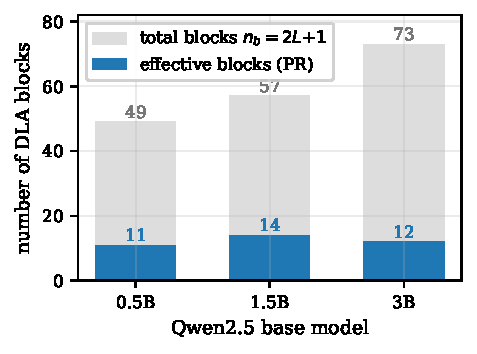
\includegraphics[width=0.92\columnwidth]{figures/rank_concentration.pdf}
\caption{Rank concentration across scale (Qwen2.5 base, prose). The effective number
of blocks driving the decode stays $\sim$constant ($\sim$12) while the total block
count $\nb=2L{+}1$ grows, so rank slack grows with scale.}
\label{fig:rank}
\end{figure}

\begin{table}[t]
\caption{Real-model routing across scale (Qwen2.5 base, prose). PR$/\nb\ll1$ is rank
concentration; $\mu/$Welch $\gg1$ is coherence slack.}
\label{tab:scale}
\small
\begin{tabular}{lcccccc}
\toprule
model & $\nb$ & recon & PR$/\nb$ & $\mu$ & $\mu/$Welch & margin \\
\midrule
0.5B & 49 & 1.00 & 11/49 & 0.268 & 2.01 & 1.24 \\
1.5B & 57 & 1.00 & 14/57 & 0.261 & 2.18 & 1.27 \\
3B   & 73 & 1.00 & 12/73 & 0.339 & 3.62 & 1.30 \\
\bottomrule
\end{tabular}
\end{table}

Moreover the concentration is not a different random subset each token: the global
participation ratio over the mean per-block contribution tracks the per-position
ratio (e.g.\ 14.8 vs.\ 11.4 for 0.5B), and the global top-12 blocks capture 73--78\%
of per-position decode mass (Table~\ref{tab:circuit}). The effective routing is a
\emph{stable, identifiable circuit}, concentrated in late layers (78--85\% of mass)
and dominated by MLP blocks (73--84\%). Rank concentration is thus a structural
property---a small late-MLP read-out circuit---not merely a per-token statistic.

\begin{table}[t]
\caption{The effective blocks form a consistent late-MLP circuit (Qwen2.5 base,
prose). Global PR $\approx$ per-position PR, and the global top-12 blocks carry most
of the per-position decode mass.}
\label{tab:circuit}
\small
\begin{tabular}{lccccc}
\toprule
model & per-pos PR & global PR & top-12 mass & late & MLP \\
\midrule
0.5B & 11.4 & 14.8 & 75\% & 78\% & 76\% \\
1.5B & 14.0 & 17.9 & 73\% & 81\% & 73\% \\
3B   & 11.8 & 15.0 & 76\% & 85\% & 78\% \\
\bottomrule
\end{tabular}
\end{table}

The same analysis on the Pythia suite (Table~\ref{tab:scalepythia})---a second
pretraining corpus (the Pile) and architecture (GPT-NeoX)---confirms rank
concentration in a different family: PR$\,\ll\nb$ throughout, again on a
\emph{consistent} circuit (global PR $\approx$ per-position PR), late- and
MLP-leaning. The scale \emph{trend} differs from Qwen, however. The smallest Pythia
models concentrate hardest---$\sim$3 of 13--25 blocks, with a large embedding share
(30--37\% of decode mass) and 97\% of mass in the late third---and the effective
count \emph{rises} with size to $\sim$14--21. So the cross-family invariant is rank
concentration itself, not Qwen's near-constant $\sim$12. The axis on which the
families genuinely part ways is coherence (the $\mu/$Welch column), which we take up
next.

\begin{table}[t]
\caption{Real-model routing across scale on Pythia (Pile, GPT-NeoX; prose). Rank
concentration (PR$/\nb\ll1$) transfers, but coherence packing $\mu/$Welch is
\emph{near-optimal} (1.06--1.5$\times$), unlike Qwen (Table~\ref{tab:scale}).}
\label{tab:scalepythia}
\small
\begin{tabular}{lcccccc}
\toprule
model & $\nb$ & recon & PR$/\nb$ & $\mu$ & $\mu/$Welch & margin \\
\midrule
70M  & 13 & 1.00 & 2.9/13  & 0.289 & 1.06 & 0.98 \\
160M & 25 & 1.00 & 2.6/25  & 0.269 & 1.39 & 1.11 \\
410M & 49 & 1.00 & 20.7/49 & 0.184 & 1.38 & 1.18 \\
1B   & 33 & 1.00 & 13.9/33 & 0.249 & 1.50 & 1.21 \\
\bottomrule
\end{tabular}
\end{table}

\subsection{Coherence packing is family-dependent}
\label{sec:cohreal}
Treat each position's decode-vs-runner-up direction in block space as a routing
feature, and measure their mutual coherence $\mu$ against the Welch floor
$\sqrt{(N-\nb)/(\nb(N-1))}$ (Theorem~\ref{thm:welch}; Fig.~\ref{fig:coh}). Here the
two families diverge, and the divergence is the single sharpest signal in the
real-model data. \emph{Qwen leaves substantial slack}---$\mu/$Welch sits
2--3.6$\times$ above the floor in every condition ($\mu\approx0.26$--$0.41$).
\emph{Pythia does not}: it packs near-optimally, $\mu/$Welch $=1.06$--$1.5\times$,
hugging the same floor a task-specialized synthetic learner reaches.

The cleanest comparison controls the dimension. At $\nb{=}49$ and $N\approx380$
(identical routing-feature geometry), Pythia-410M packs at $1.38\times$ Welch
($\mu{=}0.18$) while Qwen2.5-0.5B sits at $2.01\times$ ($\mu{=}0.27$)---a genuine
difference in realized coherence, not a floor artifact. So near-Welch-optimal
packing, which we previously observed only in task-specialized SGD
(\S\ref{sec:routing}), \emph{does} occur in a general pretrained family: it is a
property of the training recipe (corpus, optimizer, regularization), not a universal
consequence of pretraining. The structural bound holds for both families: the Welch
floor is real and never violated. What differs---and what the diagnostic
measures---is how much slack each family leaves above it, and that separates Qwen
from Pythia cleanly (Fig.~\ref{fig:coh}). (The smallest Pythia models have small
$\nb$ and thus a high floor with little room to be loose, so the $\nb{=}49$
comparison is the controlled one.)

\begin{figure}[t]
\centering
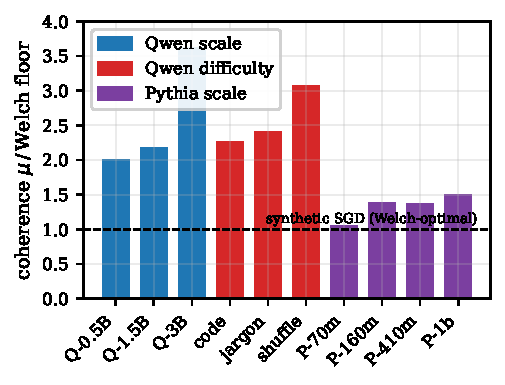
\includegraphics[width=0.95\columnwidth]{figures/coherence_slack.pdf}
\caption{Coherence relative to the Welch floor, by family. A task-specialized
synthetic learner packs to $\sim$1$\times$ (dashed line). Qwen2.5 (scale and
difficulty conditions) sits 2--3.6$\times$ above it; Pythia hugs it
(1.06--1.5$\times$). Near-optimal packing is thus family-dependent, not synthetic-specific.}
\label{fig:coh}
\end{figure}

\subsection{Difficulty increases slack via fallback}
\label{sec:diffreal}
Is the slack an easy-corpus artifact? We varied input difficulty (using the model's
own decode margin as the proxy). The result is the \emph{opposite} of the naive
expectation (Table~\ref{tab:diff}). The genuinely hard corpus (shuffled word order,
margin $0.48$) gives the \emph{most} slack: fewer effective blocks ($9/49$) and
looser packing ($\mu{=}0.41$). The mechanism is fallback---a confused model leans on
a few generic high-prior blocks. (Code is a red herring: its rigid syntax makes the
model \emph{more} confident, margin $2.56$; rare-word jargon is mostly
retrieval-style subword completion.) So the rank slack and looseness are intrinsic
and \emph{grow} with difficulty.

\begin{table}[t]
\caption{Difficulty dial (Qwen2.5-0.5B-Instruct). Harder inputs (lower margin)
produce \emph{more} slack: fewer effective blocks, looser packing.}
\label{tab:diff}
\small
\begin{tabular}{lcccc}
\toprule
corpus & margin ($\downarrow$ harder) & PR$/\nb$ & $\mu$ & $\mu/$Welch \\
\midrule
prose (easy)      & 1.24 & 11/49 & 0.268 & 2.01 \\
code              & 2.56 & 12/49 & 0.288 & 2.27 \\
rare-word jargon  & 1.74 & 9/49  & 0.305 & 2.41 \\
shuffled (hard)   & 0.48 & 9/49  & 0.407 & 3.07 \\
\bottomrule
\end{tabular}
\end{table}

\paragraph{Multilingual robustness.}
The picture is qualitatively robust across five languages (English, Chinese, French,
German, Spanish): all reconstruct $1.00$, routing stays rank-concentrated
($\sim$7--11 of 49 blocks), and coherence stays in the Qwen-typical loose band,
slightly looser for the less-fluent languages---consistent with the difficulty
finding. The per-language numbers are deferred to Appendix~\ref{app:multilingual}.

\section{Discussion}
\label{sec:discussion}

The near-term value of PIC and TRC is \emph{diagnostic}, not algorithmic: measuring
rank concentration, identifying the read-out circuit, quantifying coherence slack,
and detecting difficulty-driven fallback---quantities a practitioner can read off a
frozen model with a faithful DLA seam, and which behave lawfully across scale,
difficulty, and language. The rest of this section explains why the framework lands
on the diagnostic side of that line, and why that is the right place for it.

Combining the proved structural bounds (Theorems~\ref{thm:sep}--\ref{thm:welch}) with
the synthetic and real measurements yields a coherent picture. \emph{Cell capacity
is not the operative limit}: it is slack by $\sim$50--59 orders of magnitude
(\S\ref{sec:scored}), and both real-model families confirm large rank slack
(\S\ref{sec:real}). The operative quantity is \emph{TRC}, and it is a superposition
quantity---how many routing features a budget of $M$ generators can pack with
tolerable interference (\S\ref{sec:routing}). On the synthetic substrate, plain SGD
already performs that packing near the Welch floor, which is exactly why the four
theory-guided interventions are null: there is no slack for them to recover. The
contribution of the theory there is not a better optimizer but the \emph{ceiling and
the coordinates}---what is reachable, and in which basis.

Real models then sort into two regimes the diagnostic makes visible. \emph{Rank
concentration transfers universally}: both Qwen and Pythia route through a small,
stable, late-MLP circuit, the empirical face of the rank bound
(Theorem~\ref{thm:rank}). \emph{Coherence packing does not}: Qwen leaves 2--3$\times$
slack above the Welch floor, whereas Pythia packs near it (1.06--1.5$\times$), as
tightly as task-specialized synthetic SGD. We had initially read near-optimal packing
as a signature of task specialization that general pretraining would not pay for; the
Pythia result refutes that and is the more interesting finding. Whether a family packs
its routing features tightly is a property of the \emph{training recipe}---corpus,
optimizer, regularization---not a universal consequence of pretraining, and not
something accuracy or loss curves reveal. PIC is the instrument that surfaces it: a
single scalar, $\mu/$Welch, that cleanly separates two model families trained to
comparable competence.

\section{Related work}

\subsection{Tropical geometry and neural networks}
\citet{zhang2018tropical} established the foundational connection between feedforward
ReLU networks and tropical geometry, showing that such networks compute tropical
rational maps, with decision boundaries corresponding to tropical hypersurfaces and
linear regions to vertices of associated Newton polytopes. This has been extended to
real tropical geometry~\cite{brandenburg2024real} and applied to decision-boundary
analysis~\cite{alfarra2023decision} and linear-region
counting~\cite{montufar2014regions,serra2018regions}. \emph{All of this prior work
addresses the input--output map of feedforward classifiers.} We instead apply
tropical geometry to the \emph{routing and read-out behavior of decoder-only
transformers}, via direct logit attribution. The relevant geometric object is then
the Laguerre power diagram of the affine logit functions, and the central structural
result is a $\gamma$-code packing \emph{count} on confidently decodable tokens
(Corollary~\ref{cor:packing})---the decision-side analogue of the Welch coherence
bound rather than a region count.

\subsection{Superposition in neural networks}
Our coherence analysis provides a routing-side instance of superposition. A network
can represent more features than it has dimensions only by accepting interference, and
that interference is bounded below by coherence measures such as the Welch
bound~\cite{welch1974lower}. This is the lens of toy-model and complexity-theoretic
work on superposition~\cite{elhage2022superposition,adler2024superposition}, which
has focused on \emph{hidden representations}. We extend the same accounting to the
\emph{routing} side. When the number of routing features $n$ exceeds the effective
dimension $M$ of the rule-activation space, their coherence is Welch-floored
(Theorem~\ref{thm:welch}). We further show empirically that gradient descent attains
near-optimal packing ($\sim$1$\times$ the floor) on task-specific substrates, whereas
general pretrained models leave measurable slack (2--3$\times$ the floor) on
naturally occurring routing features (\S\ref{sec:routing}--\ref{sec:real}). Routing,
in other words, is superposition with $M$ as the packing dimension.

\subsection{Low-rank and routing in transformers}
Efficiency-oriented work explores low-rank and sparse approximations to
attention~\cite{chen2021scatterbrain} to reduce computational cost. Our contribution
is complementary and orthogonal: we \emph{measure} naturally occurring rank
concentration in the routing behavior of pretrained models as an emergent structural
property, rather than imposing low-rank structure for efficiency.

\subsection{Mechanistic interpretability and incidence calculus}
Our analysis builds on direct logit attribution and the residual-stream view of
transformer circuits~\cite{elhage2021framework,nostalgebraist2020logitlens}. On top
of that additive decomposition we introduce a geometric and logical semantics
(incidence calculus plus tropical geometry) together with a capacity theory
(Tropical Realization Complexity), and we modernize classical incidence
calculus~\cite{bundy1985incidence,liu1996incidence} for the inner-product structure
of transformer residuals---replacing world-sets with signed incidences and
structural overlap with a Gram kernel.

\section{Limitations and threats to validity}

The real-model analysis rests on one design choice---``routing feature =
decode-vs-runner-up direction in block space''---which is reasonable but not unique;
alternative definitions could shift the coherence numbers. The DLA blocks are
\texttt{fieldrun}'s decomposition, not the only circuit basis. Non-English samples
are small ($N{=}96$--127), so per-language coherence is noisy (the qualitative trend
is the signal). The synthetic substrate is deliberately stylized (planted clusters,
XOR coding); its value is a controllable ground truth, not ecological realism. The
machine-checked results (Theorems~\ref{thm:softmax}--\ref{thm:welch}) are verified in
the \texttt{i-orca} corpus~\cite{iorca}; the packing constant in
Corollary~\ref{cor:packing} is the standard covering-number corollary of
Theorem~\ref{thm:sep}. Finally, we cover two families (Qwen2.5 and Pythia): they
already show that coherence packing is family-dependent rather than universal, so
single-family conclusions about packing should not be generalized---identifying what
in a training recipe sets the packing tightness, across more families and corpora,
remains open.

\section{Conclusion and future work}

We presented Projective Incidence Calculus as a geometric and logical account of
transformer decision making, together with Tropical Realization Complexity as a
diagnostic for routing cost. We proved the structural backbone---exact decode
recovery, a decode-separation/packing bound, generator rank, and a routing Welch
floor---in a machine-checked corpus. A deliberate set of four null interventions then
showed that the framework's value is diagnostic rather than algorithmic: capacity is
hugely slack, and SGD already packs near the floor. Across two model families,
real-model analysis then shows that rank-concentrated routing on a stable late-MLP
circuit is universal, whereas coherence packing is \emph{family-dependent}---loose in
Qwen (2--3$\times$ Welch), near-optimal in Pythia (1.06--1.5$\times$).

Future directions include: practical estimators for TRC on large models; whether
narrow fine-tuning tightens packing toward the synthetic ($\sim$1$\times$) regime;
hybrid generation that activates only when diagnostics indicate rank or interference
pressure; and---prompted by the Qwen/Pythia split---identifying which ingredients of
a training recipe set routing-packing tightness, across more families and corpora.
All code, formal certificates, and results are available in the \texttt{fieldrun},
\texttt{i-orca}, and \texttt{pil} repositories.

\bibliographystyle{ACM-Reference-Format}
\bibliography{references}

\appendix

\section{Multilingual routing detail}
\label{app:multilingual}
Table~\ref{tab:lang} reports the per-language routing numbers for
Qwen2.5-0.5B-Instruct on matched content, supporting the robustness claim in
\S\ref{sec:diffreal}. All five languages reconstruct the decode $1.00$ of the time,
route through $\sim$7--11 of 49 blocks, and show $\mu\approx0.27$--0.36. Non-English
is slightly \emph{more} concentrated and looser, consistent with the difficulty
finding (marginally lower fluency $\to$ more fallback); Chinese matches English
coherence ($\mu{=}0.269$) despite the script. Non-English $N$ is small (96--127), so
$\mu$ is noisier; the qualitative picture is the signal.

\begin{table}[h]
\caption{Multilingual routing (Qwen2.5-0.5B-Instruct, matched content, $\nb=49$).}
\label{tab:lang}
\small
\begin{tabular}{lccc}
\toprule
language & PR$/\nb$ & $\mu$ & margin \\
\midrule
en & 11/49 & 0.268 & 1.24 \\
zh & 8/49  & 0.269 & 1.12 \\
fr & 8/49  & 0.329 & 1.89 \\
de & 8/49  & 0.357 & 1.54 \\
es & 7/49  & 0.343 & 1.99 \\
\bottomrule
\end{tabular}
\end{table}

\end{document}
